\chapter{Previous Work} \label{ch:prev}

This chapter covers previous work in the area of canonical
representations of functions, word-level abstractions and their
application to design verification. Since the application of our
approach is targeted towards formal equivalence verification, modern
combinational equivalence checking techniques are also
reviewed. Finally, formal verification techniques using computer
algebra, algebraic geometry, and polynomial interpolation are also
considered. 

\section{Canonical Decision Diagrams}
Canonical representations of Boolean functions have been the subject
of extensive investigation for logic synthesis and design
verification. The Reduced Ordered Binary Decision Diagram (ROBBD)
\cite{BRYA86} was the first significant contribution in this area. 
Efficient implementation of ROBDDs as a software package \cite{brace}
allowed for efficient formal verification of combinational and
sequential circuits.  ROBDDs represent a Boolean function as an
implicit set of points on a canonical directed acyclic graph
(DAG). Manipulation of Boolean functions can then be carried out as
composition operations on their respective DAGs.  The decomposition
principle behind BDDs is one of Shannon's expansion, i.e.
\begin{equation}
f(x, y, \dots) = x f_x + x' f_{x'}
\end{equation}

where $f_x = f(x = 1)$ and $f_{x'} = f(x = 0)$ denote the positive and
negative co-factors of $f$ w.r.t. $x$, respectively. Motivated by the
success of BDDs,  variants of the Shannon's decomposition principle
(Davio, Reed-Muller, etc.) were explored to develop other functional
decision diagrams. For example, the AND-OR-NOT logic based Shannon's
expansion is transformed into an AND-XOR logic based decomposition,
termed as the Davio's decomposition:

\begin{eqnarray}
f(x, y, \dots) &=& x f_x + x' f_{x'}\\
& = & x f_x \oplus x' f_{x'}\\
& = & x f_x \oplus (1 \oplus x) f_{x'}\\
& = & f_{x'} \oplus x (f_x \oplus f_{x'})
\end{eqnarray}


Decision diagrams based on such decompositions include FDDs
\cite{okfdd}, ADDs \cite{add}, MTBDDs \cite{mtbdd}, and their hybrid 
edge-valued counterparts, HDDs \cite{hdd} and EVBDDs \cite{evbdd}. 
While these are referred to as {\it Word-Level Decision Diagrams}
\cite{WLS}, the decomposition is still point-wise, binary, 
w.r.t. each Boolean variable. These representations do not
serve the purpose of word-level abstraction from bit-level
representations. 

Binary Moment Diagrams (BMDs) \cite{bmd}, and its derivatives K*BMDs
\cite{kbmd} and *PHDDs \cite{phdd}, depart from the Boolean
decomposition and perform the decomposition of a {\it linear} function
based on its two moments. BMDs provide a compact representation for
integer arithmetic circuits such as multipliers and squarers. However,
these are inapplicable to word-level abstraction of modulo-arithmetic
circuits over Galois fields. 
%in our application, we encounter modulo-arithmetic circuits and that
%too over Galois fields. For such applications, these representations
%are inapplicable. Taylor Expansion Diagrams (TEDs) \cite{ted_tcomp}
%generalize the linear moment decomposition of BMDs into a Taylor
%series expansion --- this allows the representation of RTL
%descriptions as polynomials over bit-vectors. However, 


Taylor Expansion Diagrams (TEDs) \cite{ted_tcomp} are a
word-level canonical representation of a {\it polynomial expression},
based on the Taylor's series expansion of a polynomial. However, they do
not represent a {\it polynomial function} canonically. For example,
$f_1 = 0$ and $f_2 = 2x^2 - 2x \pmod{ 4}$ are two different polynomial
representations of the zero function over $\Z_4$; but they are
symbolically different polynomials and they have non-isomorphic TED
DAGs.  While \cite{namrata:phd}  and \cite{alizadeh:tcad2010} provide 
canonical representations of polynomial functions, they do so over
finite integer rings $\Z_{2^k}$ and not over Galois fields $\Fkk$.


MODDs \cite{modd} \cite{modd_tcomp} are a DAG representation of the
characteristic function of a circuit over Galois fields $\Fkk$. MODDs
come very close to satisfying our requirements as a canonical
word-level representation that can be employed over Galois fields, as
it essentially interpolates a polynomial from the characteristic 
function. However, MODDs do not scale very well for large circuits ---
this is because every node in the DAG can have up to $k$ children and
the normalization operations are very complicated for MODDs. They also
suffer from the size explosion problem during intermediate
computations. They are known to be infeasible in representing
functions over $32$-bit operand words. 

\section{Word-Level Techniques in RTL Synthesis and Verification}

Other attempts to derive high-level representations of functions,
along with associated decision procedures, can be found in
the rich domain of formal model checking \cite{BHEL96} \cite{SMV},
theorem proving \cite{arditi:bmd}, bit-vector SMT-solvers
\cite{boolector} \cite{cvc3} \cite{z3} \cite{bitvector98}, automated
decision procedures for Presburger arithmetic \cite{presburger}
\cite{bultan:mixed_verification}, algebraic manipulation techniques 
\cite{devadas:algebraic_manipulation_iccd91}, or the ones based on
term re-writing \cite{AST}, etc. 
%Other forms of high-level logics,
%such as EUF \cite{Burch:CAV94}, PEUFM \cite{Velev:JSC03}
%\cite{Velev:CL01}, CLU \cite{Lahiri:CAV02} have been derived for
%verifying micro-processor pipeline control. 
Polynomial, integer and other non-linear representations have also
been researched: Difference Decision Diagrams (DDDs) \cite{ddd-csl99} \cite{ddd-mt-98}, interval
diagrams \cite{interval_dd}, interval analysis using polynomials
\cite{polynomial_sanchez99}, etc. Most of these have found 
application in constraint satisfaction for simulation-based
validation:  \cite{Ritter99} \cite{hsat} \cite{lpsat}
\cite{brinkmann:asp-dac} \cite{Huang:tcad01} \cite{bitvector98}. Among
these, \cite{brinkmann:asp-dac} \cite{Huang:tcad01} \cite{bitvector98}
have been used to {\it solve} integer modular arithmetic on linear
expressions - a different application from {\it representing}
finite field modulo-arithmetic on polynomials in a canonical form.   


\section{Combinational Equivalence Checking}

The verification problem addressed in this dissertation is a
manifestation of the combinational equivalence checking (CEC) problem,
where the specification (polynomial) and  the implementation (circuit)
are custom-designed, structurally very dissimilar circuits. To make
use of contemporary gate-level CEC tools, we can take the 
specification circuit (``golden model'') and check its equivalence
against the implementation circuit. Canonical decision diagrams (BDDs
\cite{BRYA86} and their word-level variants \cite{WLS}),
And-Invert-Graph (AIG) based reductions \cite{AIG:2002}
\cite{alanmi:cec:iccad2006}, circuit-SAT solvers \cite{csat}, etc.,
are among the many techniques that can be employed for this CEC.  
When one circuit is synthesized from the 
other, this problem can be efficiently solved using AIG-based
reductions (e.g. the ABC tool \cite{abc}) and circuit-SAT solvers
(e.g., CSAT \cite{csat}). 
Synthesized circuits generally contain many
sub-circuit equivalences which AIG and CSAT based tools can identify
and exploit for verification. However, when the circuits are
functionally equivalent but structurally very dissimilar (e.g.,
Mastrovito \cite{mastro:1989} versus Montgomery implementations
\cite{acar:1998} of Galois field circuits), none of the 
  contemporary techniques, including ABC and CSAT, offer a practical
  solution. Automatic formal verification of large {\it
    custom-designed modulo-arithmetic circuits} largely remains
  unsolved today.    

This verification problem is very hard for SAT solvers and also for
quantifier-free bit-vector (QF-BV) theory based SMT-solvers, due to
the large circuit size, and the presence of AND-XOR-SHIFT structures. 
Similarly, the Cryptol tool-set \cite{Cryptol:fmcad09} also employs
AIG-based reductions (SAT-sweeping) and SAT/SMT-solvers for
verification of crypto-protocols. For applications where
AIGs/SAT/SMT-techniques fail, the {\it Cryptol} tool-set also does not
deliver. As shown in \cite{lv:phd}, {\it none of BDDs, SAT, SMT
  solvers, nor the  ABC tool can prove design equivalence beyond
  $16$-bit circuits.}

%%%%%%%%%%MACIEJ HERE%%%%%%%%%%%%%%%
In \cite{ciesielski:flow}, the authors present a method
for verification of integer multipliers using a data-flow
approach. This work abstracts a polynomial function
of the given multiplier and then solves the network flow problem 
using algebraic techniques. However, the abstraction is 
solely bit-level, and is thus not applicable to deriving 
a word-level representation of a given design.

\section{Verification of Galois Field Circuits}

Symbolic computer algebra techniques have been employed for formal
verification of circuits over $\Z_{2^k}$ and also over
Galois fields $\Fkk$. 
The work of \cite{gao:gf-gb-ms} shows how to use Gr\"obner basis
techniques to count the zeros of an ideal $J$ over ${\mathbb{F}}_q$
(i.e. count $V_{{\mathbb{F}}_q}(J)$). The authors then follow-up with
an approach for {\it quantifier elimination} over Galois fields
${\mathbb{F}}_q$ \cite{gao:qe-gf-gb}. 
However, computing a \Grobner basis is computationally
expensive.
While these works present
the proper theory and algorithms, 
efficiency/improvements to the Gr\"obner
basis computation is not addressed. This is also the case with other
general verification techniques using Gr\"obner bases
\cite{Avrunin:CAV} \cite{gbverify:2007} \cite{manna:program}, etc. 
%The paper \cite{wienand:cav08} addresses verification of %-TIM
%finite-precision integer datapath circuits using the concepts of %-TIM
%Gr\"obner bases over the ring ${\mathbb{Z}}_{2^k}$. %-TIM
%They model the
%circuit constraints by way of arithmetic-bit-level (ABL) polynomials
%($\{G\}$) and formulate the verification test as an equivalent
%{\it variety subset problem}. To solve this, first they derive a term
%order to represent the circuit polynomials $\{G\}$ with a Gr\"obner
%basis. Then they compute a normal form $f$ of the specification $g$
%w.r.t. $\{G\}$. They show that, under certain constraints that are
%satisfied by their term order, the circuit is correct if and only if
%$f$ is a vanishing polynomial over ${\mathbb{Z}}_{2^k}$
%\cite{shekhar:tcad07}. 
%In \cite{wedler:date11}, the authors further                 %-TIM
%show an integration of their approach within an SMT-solver for %-TIM
%arithmetic instances.                        %-TIM
%show that  the vanishing polynomial test can be
%omitted by formulating the problem directly over $Q :=
%{\mathbb{Z}}_{2^k} [X]/\langle x^2-x : x \in X \rangle$. 

In \cite{ibm:ecc-ita11} \cite{blueveri:ita} \cite{ibm:blueveri},
%from IBM needs special mention: T
the authors present the {\sc BLUEVERI} tool from IBM for verification
of Galois field circuits for error correcting codes against an
algorithmic spec. The implementation consists of a set of
(pre-designed and verified) circuit blocks that are interconnected to
form the error correcting system. The spec is given as a set of design
constraints on a ``check file''. Their objective is to prove the 
equivalence of the implementation against this check file.
They model the verification instance as a data-flow graph, represent each
sub-circuit block with its known (word-level) polynomial over $\Fq$,
and formulate the verification problem using the {\it Weak
  Nullstellensatz} --- i.e. to check if the {\it variety} of the
algebraic system ``{\it spec} $\neq$ {\it implementation}'' is empty
for which they employ a Nullstellensatz formulation.
%for which they use a Gr\"obner basis engine. 
Their main
contributions are: i) a ``term re-writing'' to specify the algorithmic
description using polynomials (ideal); and ii) integrating an
AIG-style \cite{AIG:2002} Boolean solver with their word-level
decision procedure, with lazy signal computations and Boolean
reasoning. For final verification, the polynomial system is given
to a computer algebra tool ({\sc Singular} \cite{DGPS}) to {\it
  compute} a reduced Gr\"obner basis. However, improvements to the
core Gr\"obner basis computational engine are not the subject of their
work.   

In \cite{lv:phd} 
\cite{lv:tcad2013}
\cite{lv:date2012}
\cite{lv:hldvt2011} \cite{lv:vlsi2012}, {\it Lv et al.} present
computer algebra techniques for formal verification of Galois field
arithmetic circuits. Given a specification polynomial $f$, and a
circuit $C$, they formulate the verification problems as an ideal
membership test using the Strong Nullstellensatz and Gr\"obner
bases. In \cite{lv:date2012}, the authors show that for any
combinational circuit, {\it there exists a term order $>_1$ that
  renders the set of polynomials of the circuit itself a Gr\"obner
  basis --- and this term order can be easily derived 
by performing a topological traversal of the circuit}. By exploiting
this term order, verification can be significantly scaled
to $163$-bit (NIST-specified) cryptography circuits. 
In contrast to the work of \cite{lv:phd}, we are not given a
specification polynomial. Instead, given the circuit $C$, we want
to derive (extract) the word-level specification $f$. In our work, we
borrow and further build upon the results of \cite{gao:gf-gb-ms}
\cite{gao:qe-gf-gb} %\cite{modd_tcomp} 
\cite{lv:date2012} \cite{lv:phd}. 

\section{Verification of Integer Arithmetic Circuits using Gr\"obner Bases}
Symbolic computer algebra techniques have been used for verification
of integer arithmetic circuits \cite{wienand:cav08} and also for
decision procedures over Galois fields \cite{gao:gf-gb-ms}. The paper
\cite{wienand:cav08} addresses verification of finite precision
integer datapath circuits using the concepts of  Gr\"obner bases over
the ring ${\mathbb{Z}}_{2^k}$. This work models the circuit constraints by
way of arithmetic-bit-level (ABL) polynomials ($\{G\}$), and formulates
the verification test as an equivalent variety subset problem. This problem
is solved by deriving a term order that already makes $\{G\}$
a Gr\"obner basis, then computing a normal form $f$ of the
specification $g$ w.r.t. $\{G\}$. Circuit correctness is established
by testing whether or not $f$ is a vanishing
polynomial over ${\mathbb{Z}}_{2^k}$ \cite{shekhar:tcad07}.
In \cite{wedler:date11}, the
authors further show that the vanishing polynomial test can be omitted
by formulating the problem directly over $Q := {\mathbb{Z}}_{2^k}
[X]/\langle x^2-x : x \in X \rangle$.  
However, in these works, the problem requires that the word-level 
abstraction of the circuit be known, whereas our approach derives 
this abstraction polynomial. 

\section{Polynomial Interpolation in Symbolic Computation}

The problem of polynomial interpolation is a fundamental problem in
symbolic and algebraic computing which finds application in modular
algorithms, such as the GCD computation and polynomial
factorization. The problem is stated as follows: Given $n$ distinct
data points $x_1, \dots, x_n$, and their evaluations at these points
$y_1, \dots, y_n$,  {\it interpolate} a polynomial $\Func(X)$ of degree
$n-1$ (or less) such that $\Func(x_i) = y_i$ for $1 \leq i \leq n$. 
Let $t$ be the number of non-zero terms in $\Func$ and let $T$ be the
total number of possible terms. When ${{t} \over {T}} << 1$, the
polynomial $\Func$ is {\it sparse}, otherwise it is {\it dense}. Much of
the work in polynomial interpolation addresses sparse 
interpolation using the ``black-box'' model (also called the
algebraic circuit model) as shown in Fig. \ref{fig:blackbox}. 

\begin{figure}[hbt]
\centerline{
%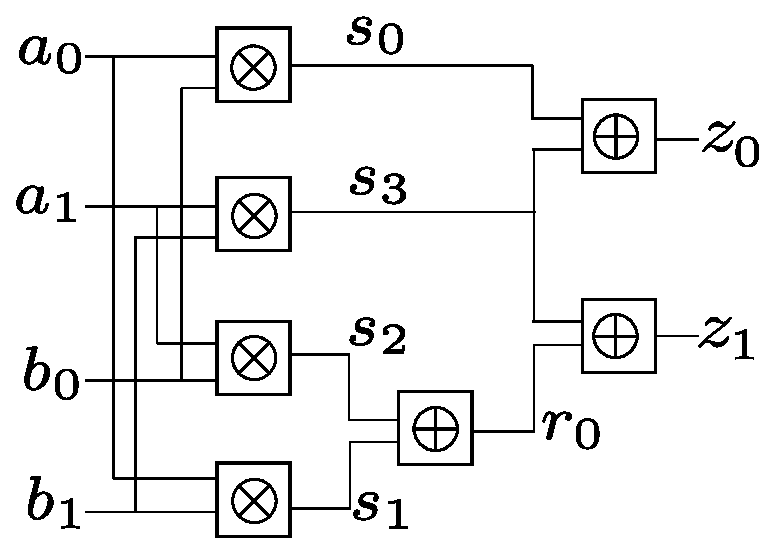
\includegraphics[scale=0.3]{../figures/2bitmultiplier.eps}
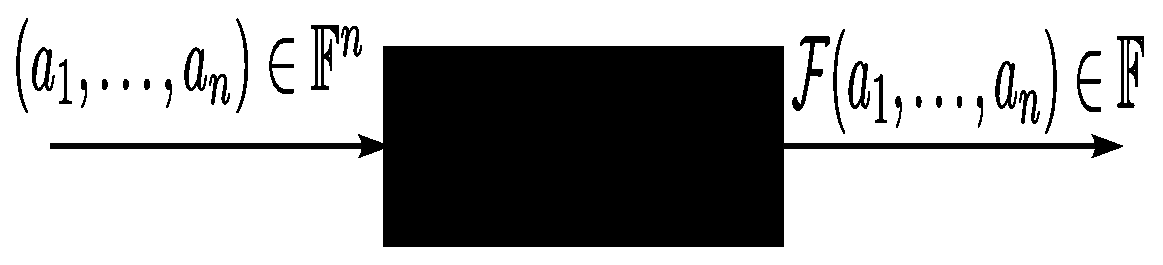
\includegraphics[scale=0.45]{figures/blackbox.eps}
}
\caption{The black-box or the algebraic circuit representation.}
\label{fig:blackbox}
\end{figure}

Let $\Func$ be a multivariate polynomial in $n$ variables $\{x_1, \dots,
x_n\}$, with $t$ non-zero terms ($0 < t < T$), represented with a
black-box $B$. On input $(x_1, \dots, x_n)$,
the black-box evaluates $y_i = \Func(x_1, \dots, x_n)$. Given also a
degree bound $d$ on $\Func$, the goal is to interpolate the polynomial
$\Func$ with a minimum number of {\it probes} to the black-box. The early
work of Zippel \cite{zippel:interpolate} and
Ben-Or/Tiwari \cite{ben-or-tiwari:interpolate} require $O(ndt)$ and
$O(T \log n)$ probes, respectively, to the black-box. These bounds
have since been improved significantly; the recent algorithm of
\cite{monagan:interpolate} interpolates with $O(nt)$ probes.  

Our problem of polynomial abstractions of Galois field circuits 
falls into the category of dense interpolation, as we
require a polynomial that describes the function at each of the $q$
points of the field $\Fq$. Newton's interpolation technique, with the
black-box model, bounds the number of probes by $(d+1)^n$ --- which 
exhibits very high complexity. In the logic synthesis area, the work of
\cite{zilic:interpolate} investigates dense interpolation. Due to this
high-complexity, their approach is feasible only for applications over
small fields, {\it e.g.} computing  Reed-Muller forms for multi-valued
logic over $\F_2$.  

For our problem,
we can also employ the black-box model by replacing the black-box
(algebraic circuit) by the given circuit $C$; then every {\it probe}
of the black-box would correspond to a {\it simulation of the
  circuit}. However, as we desire a polynomial representation of the entire
function over the Galois field, exhaustive simulation would be required, 
which is infeasible.

\section{Concluding Remarks}

For the problem of word-level, canonical, polynomial abstractions
of Galois field arithmetic circuits over $\Fkk$, previous related work 
is either inapplicable or only applicable to circuits no larger than
$32$-bits in size.
Therefore, we propose a {\it symbolic approach} to
polynomial interpolation from a circuit using the Gr\"obner basis
computation. However, the complexity of a \Grobner basis computation is 
prohibitively expensive; thus, we propose further improvements to this 
approach by deriving a smaller subset of computations based on a \Grobner
basis analysis. These improvements allow for abstractions of 
flattened Galois field circuits up to $571$-bits, which is the largest NIST 
standard for ECC, or up to $1024$-bits when a hierarchy is given. 
Furthermore, we propose applications of this 
approach to allow for formal verification of flattened Galois field circuits up to 
$1024$-bits, where current techniques are only applicable for circuits up 
to $163$-bits.
